\chapter{Ko-Sched的设计与实现}\label{chapter:design-implementation}

为解决
\begin{enumerate*}[label=\roman*),itemjoin={\quad}]
    \item 开发人员实现可分割kernel的困难
    \item 内核分割的最佳分割参数难以确认
\end{enumerate*}
,我们提出 \emph{ko-Sched},一个帮助CUDA编程人员利用kernel联合调度实现性能提升的框架。它包括
\begin{enumerate*}[label=\roman*),itemjoin={\quad}]
    \item 帮助编写可调整大小内核的框架,使得开发人员能够更容易地实现可重配置的内核
    \item 一个基于搜索算法和性能分析寻找最佳的内核分割配置的工具
\end{enumerate*}
。通过搜索和分析不同的分割配置,该程序可以找到使程序执行最快的内核分割配置,为开发人员提供一种可靠的方法来优化kernel联合调度时的性能。

\section{尺寸可调整的子内核}

\begin{lstlisting}[language=C++, label=code:koschedcode, caption=Resizable kernel using ko-sched for matrix transpose, float, firstnumber=1, escapeinside={(*}{*)}]
KernelSetting pre_process() { (*\label{code:koschedcode:preprocessbeg}*)
    // data init and allocation
    const size_t msize{..};
    float *h_iData{..}, *h_oData{..}, *d_iData{..}, *d_oData{..};
    fillInputData(h_iData, ..); (*\label{code:koschedcode:initdata}*)
    dim3 dimGrid{..}, dimBlock{..};
    cudaMemcpy (d_iData, h_iData, msize, cudaMemcpyHostToDevice); (*\label{code:koschedcode:cpy}*)

    return KernelSetting { (*\label{code:koschedcode:kernelsettingbeg}*)
        dimGrid, dimBlock, KernelArgs{d_Odata, d_iData}, 
        Context{d_Odata, d_iData, msize}
    }; (*\label{code:koschedcode:kernelsettingend}*)
}(*\label{code:koschedcode:preprocessend}*)

__global__ void transpose(KernelArgs args, dim3 blockIdx) { (*\label{code:koschedcode:kernelbeg}*)
    float *odata = args.odata; float *idata = args.idata;

    int x = blockIdx.x * TILE_DIM + threadIdx.x;
    int y = blockIdx.y * TILE_DIM + threadIdx.y;
    int width = gridDim.x * TILE_DIM;
    for (int j = 0; j < TILE_DIM; j += BLOCK_ROWS)
        odata[x * width + (y + j)] = idata[(y + j) * width + x];
}
EXECUTE(transpose); (*\label{code:koschedcode:kernelend}*)

void post_process(Context context) { (*\label{code:koschedcode:postprocessbeg}*)
    cudaMemcpy(context.h_oData, context.d_oData, 
        context.msize, cudaMemcpyDeviceToHost);
    cudaDeviceSynchronize();
    // data post-processing
} (*\label{code:koschedcode:postprocessend}*)
\end{lstlisting}

为了能分析不同分割配置下的程序性能,CUDA开发人员需要编写可被灵活分割的内核。Ko-Sched将一个CUDA程序分为\texttt{pre\_process}, \texttt{kernel\_execution}和\texttt{post\_process} 3个部分。\texttt{pre\_process}包括启动kernel前的所有处理,包括输入数据的初始化、内存分配等;\texttt{kernel\_execution}部分启动并等待kernel的执行;\texttt{post\_process}包括kernel执行结束后的事务,如保存结果和释放内存。为使用Ko-Sched,开发人员需实现并注册\texttt{pre\_process}, \texttt{post\_process}函数,ko-Sched会在在内核执行前后调用它们。此外,开发人员需要提供由\texttt{EXECUTE}标识的设备函数,Ko-Sched将按照subkernel的划分策略以不同参数调用此函数。\autoref{code:koschedcode}展示了如何将\autoref{code:naivehostcudacode}, \autoref{code:naivedevicecudacode}中的程序改写为使用ko-Sched框架的内核可分割程序,包括函数\texttt{pre\_process}(\autoref{code:koschedcode:preprocessbeg}\textasciitilde\autoref{code:koschedcode:preprocessend}), 由\texttt{EXECUTE}标识的内核函数(\autoref{code:koschedcode:kernelbeg}\textasciitilde\autoref{code:koschedcode:kernelend})和\texttt{post\_process}(\autoref{code:koschedcode:postprocessbeg}\textasciitilde\autoref{code:koschedcode:postprocessend})。\texttt{pre\_process}首先初始化输入数据(\autoref{code:koschedcode:initdata}),然后将数据从主机内存拷贝到设备内存(\autoref{code:koschedcode:cpy}),最后返回一个\texttt{KernelSetting}对象,包含了kernel的启动参数(\texttt{dimGrid}, \texttt{dimBlock})、kernel的参数(\texttt{KernelArgs}对象)和\texttt{post\_process}需要的上下文信息(\texttt{Context}对象)(\autoref{code:koschedcode:kernelsettingbeg}\textasciitilde\autoref{code:koschedcode:kernelend})。Ko-Sched启动子内核时将\texttt{pre\_process}返回的\texttt{KernelArgs}对象和原kernel中相应的\texttt{blockIdx}传递给子内核。在\texttt{kernel\_execution}部分,开发人员需要使用\texttt{EXECUTE}标识一个设备函数,ko-Sched将按照subkernel的划分策略以不同启动参数调用此函数。在\texttt{post\_process}部分,开发人员需要将结果从设备内存拷贝到主机内存,然后释放设备内存。

由于改变block的维度可能导致错误的计算,ko-Sched将保持开发人员设定的block维度。由于kernel分割改变了grid的维度,为使设备函数使用的\texttt{blockIdx}同内核未分割时一致,ko-Sched将自动计算每个block在原kernel中的索引并传值至设备函数,使得开发人员无需改变原有代码即可实现可变大小内核。

\begin{figure}[htbp]
    \centering
    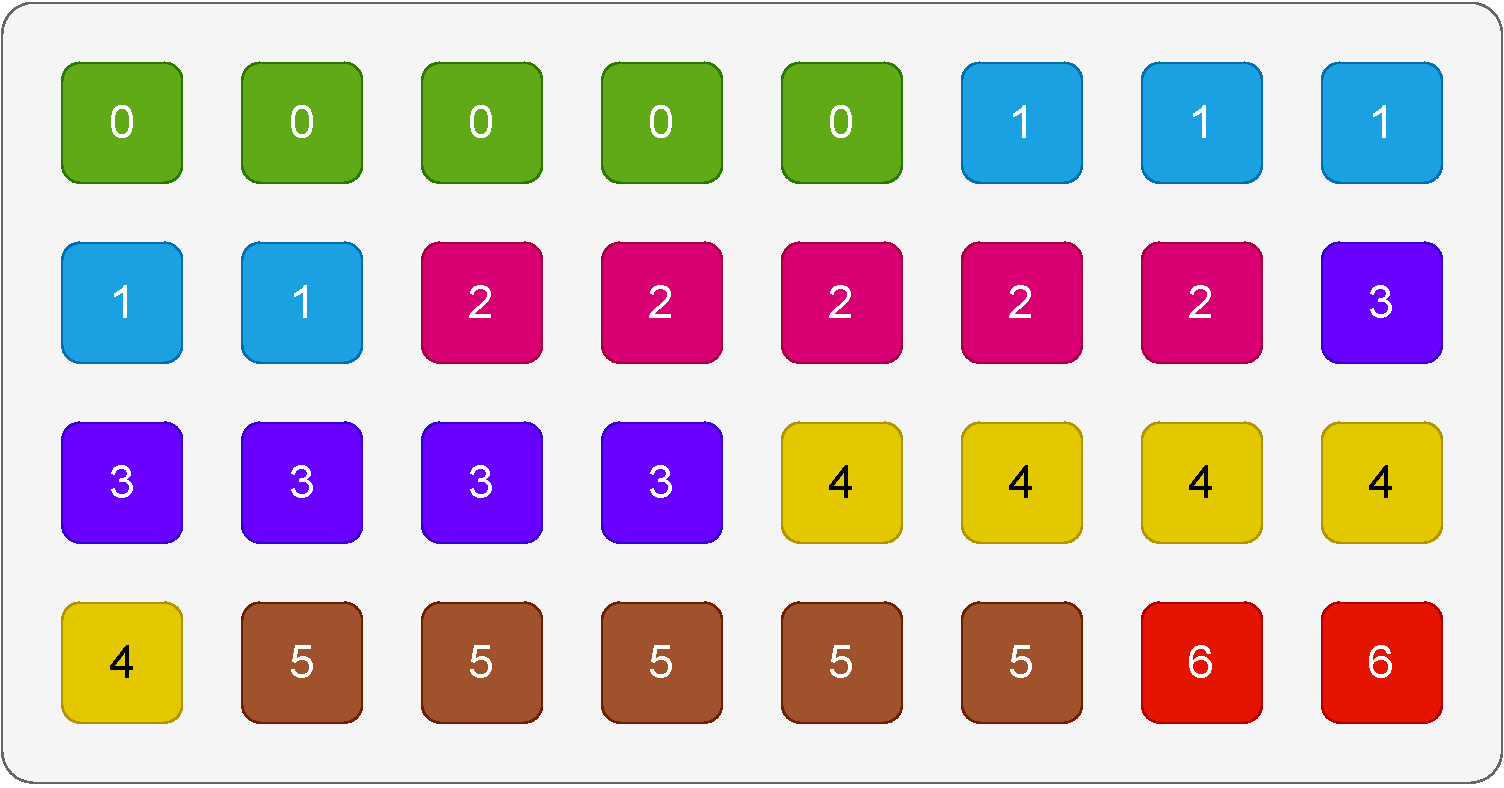
\includegraphics[width=0.8\linewidth]{kernel_division/kernel_division.drawio.pdf}
    \caption{kernel分割示意图}
    \label{kernel-division}
\end{figure}

Ko-Sched使用简单的顺序分割方式分割kernel。\autoref{kernel-division} 展示了一个二维grid所包含的blocks被划分为大小为5的子内核的方式。图中标有数字的彩色方块代表1个block,同色block被归为同一子内核,方块标注的数字为所属子内核的序号。在分割kernel时,二维grid先被顺序展开为一维,连续5个block被归为同一子内核。剩余不足5的block被归为1个较小的子内核(如子内核6)。

开发人员利用ko-Sched框架实现了可灵活分割的kernel后,ko-Sched将利用搜索算法寻找较优的分割配置。

\section{搜索算法}

\begin{algorithm}[htbp]
    \SetAlgoLined
    \KwData{初始分割参数 init\_config}
    \KwResult{搜索所得性能最佳分割参数}
    cur\_exec\_time $\gets$ estimate\_exec\_time(init\_config)\; \label{algo:searching:inittime}
    cur\_config $\gets$ init\_config\; \label{algo:searching:initconfig}
    \Loop{}{\label{algo:searching:loopbeg}
        min\_neighbor\_time $\gets$ \textbf{inf}\; \label{algo:searching:initmin}
        min\_neighbor\_config $\gets$ \textbf{null}\; \label{algo:searching:initminconfig}
        \ForEach{config $\in$ neighbors(cur\_config)}{ \label{algo:searching:neighborloopbeg}
            exec\_time $\gets$ estimate\_exec\_time(config)\; \label{algo:searching:profiletime}
            \If{exec\_time $<$ min\_neighbor\_time}{
                min\_neighbor\_time $\gets$ exec\_time\; \label{algo:searching:updatemin}
                min\_neighbor\_config $\gets$ config\; \label{algo:searching:updateconfig}
            }
        }\label{algo:searching:neighborloopend}

        \eIf{min\_neighbor\_time $<$ cur\_exec\_time}{
            cur\_exec\_time $\gets$ min\_neighbor\_time\; \label{algo:searching:updatecurtime}
            cur\_config $\gets$ min\_neighbor\_config\; \label{algo:searching:updatecurconfig}
        }{
            \Return{cur\_config}\; \label{algo:searching:return}
        }
    }\label{algo:searching:loopend}
    \caption{Subkernel Size Searching}
    \label{algo:searching}
\end{algorithm}

\autoref{consistency}展示了程序性能随内核分割参数的变化具有连续性,ko-Sched可以通过分析性能随参数变化的趋势高效寻找较优的分割参数。\autoref{algo:searching}展示了搜索算法的基本结构。\autoref{algo:searching:inittime}测试了初始参数对应的性能,其中函数\texttt{estimate\_exec\_time}估算了此配置下的性能。\autoref{algo:searching:loopbeg}\textasciitilde\autoref{algo:searching:loopend}从当前基准配置出发,对与基准配置相近的配置测试后,选择其中性能最高的配置作为新的基准配置,并不断重复此过程。其中,\autoref{algo:searching:neighborloopbeg}\textasciitilde\autoref{algo:searching:neighborloopend}对当前基准配置\texttt{cur\_config}的相似配置(由函数\texttt{neighbors}获得)依次测量性能,并将最佳性能的配置记录于\texttt{min\_neighbor\_config}(\autoref{algo:searching:updateconfig})。\autoref{algo:searching:updatecurconfig}将基准配置设置为性能最高的相近配置。若相近配置性能均低于基准配置,基准配置即为寻找到的最佳配置(\autoref{algo:searching:return})。

\begin{figure}[htbp]
    \centering
    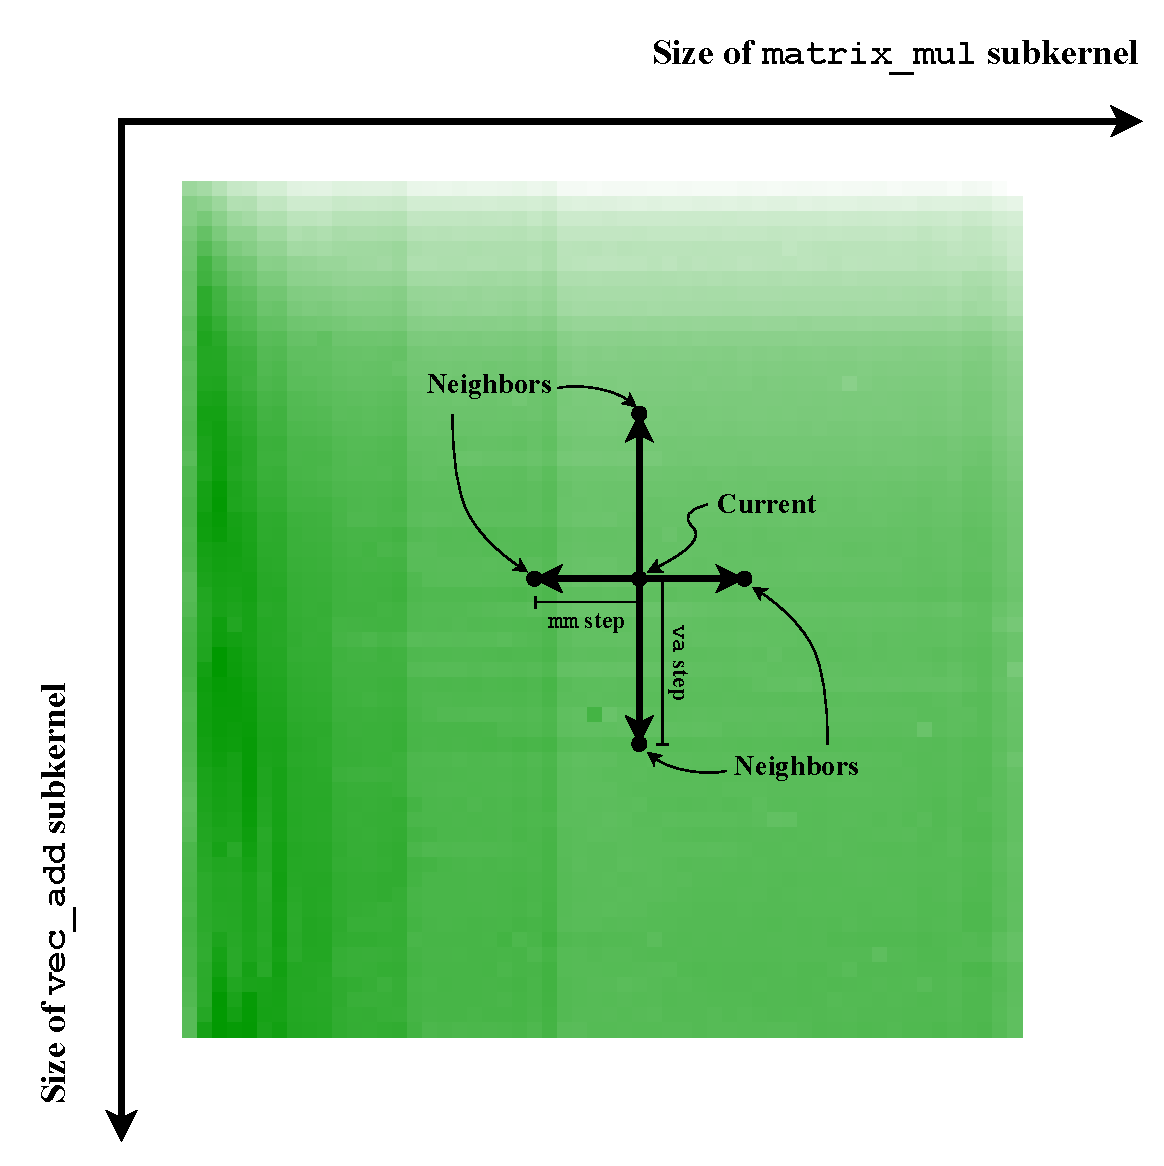
\includegraphics[width=0.8\linewidth]{searching_trace/searching_concept.drawio.pdf}
    \caption{搜索步骤示意图。"Current"为当前基准配置,"Neighbors"为相近配置。搜索算法的每一次迭代都会在当前基准配置的相近配置中选择性能最高的配置作为新的基准配置。}
    \label{searching-concept}
\end{figure}

\autoref{algo:searching} 中\autoref{algo:searching:neighborloopbeg}\textasciitilde\autoref{algo:searching:neighborloopend}的过程可由\autoref{searching-concept}的图示说明。图中标记为“Current”的配置标识当前基准配置,\texttt{neighbors}函数在基准配置周围选出若干相近配置(图中标识为“Neighbors”)。在对所有相近配置依次估算性能后,以其中性能最高者作为新的基准配置。

\subsection{相近配置的选择}

\texttt{neighbors}函数的设计对搜索效果有极大的影响。首先,\texttt{neighbors}决定了每次需测量的相近配置的数目。较大的数目允许搜索算法更高效地找到调整参数的方向,但在每一步需要测试更多的相近配置;较小的数目可以减少每次调整所需的测试数目,但选择的调整方向可能不是使性能提升最快的方向。经实验,本文默认每次选取4个方向的参数进行测试。其次,每次调整的步长的选择也十分关键。由于\texttt{estimate\_exec\_time}得到的性能估算结果有一定的波动性,区域内可能存在多个局部极值点,过小的步长会使算法收敛于局部最优解。即使未受限于局部最优解,小步长搜索会导致全程多次迭代,降低搜索效率。另一方面,过大的步长可能使算法在调整参数时忽略最优解。此外,不同内核的性能变化对参数的敏感程度不同。单一block任务量较小的kernel需要较大的分割参数改变才会有明显的性能变化,反之,单一block任务繁重的kernel的性能对参数变化较为敏感。

\begin{figure}[htbp]
    \centering
    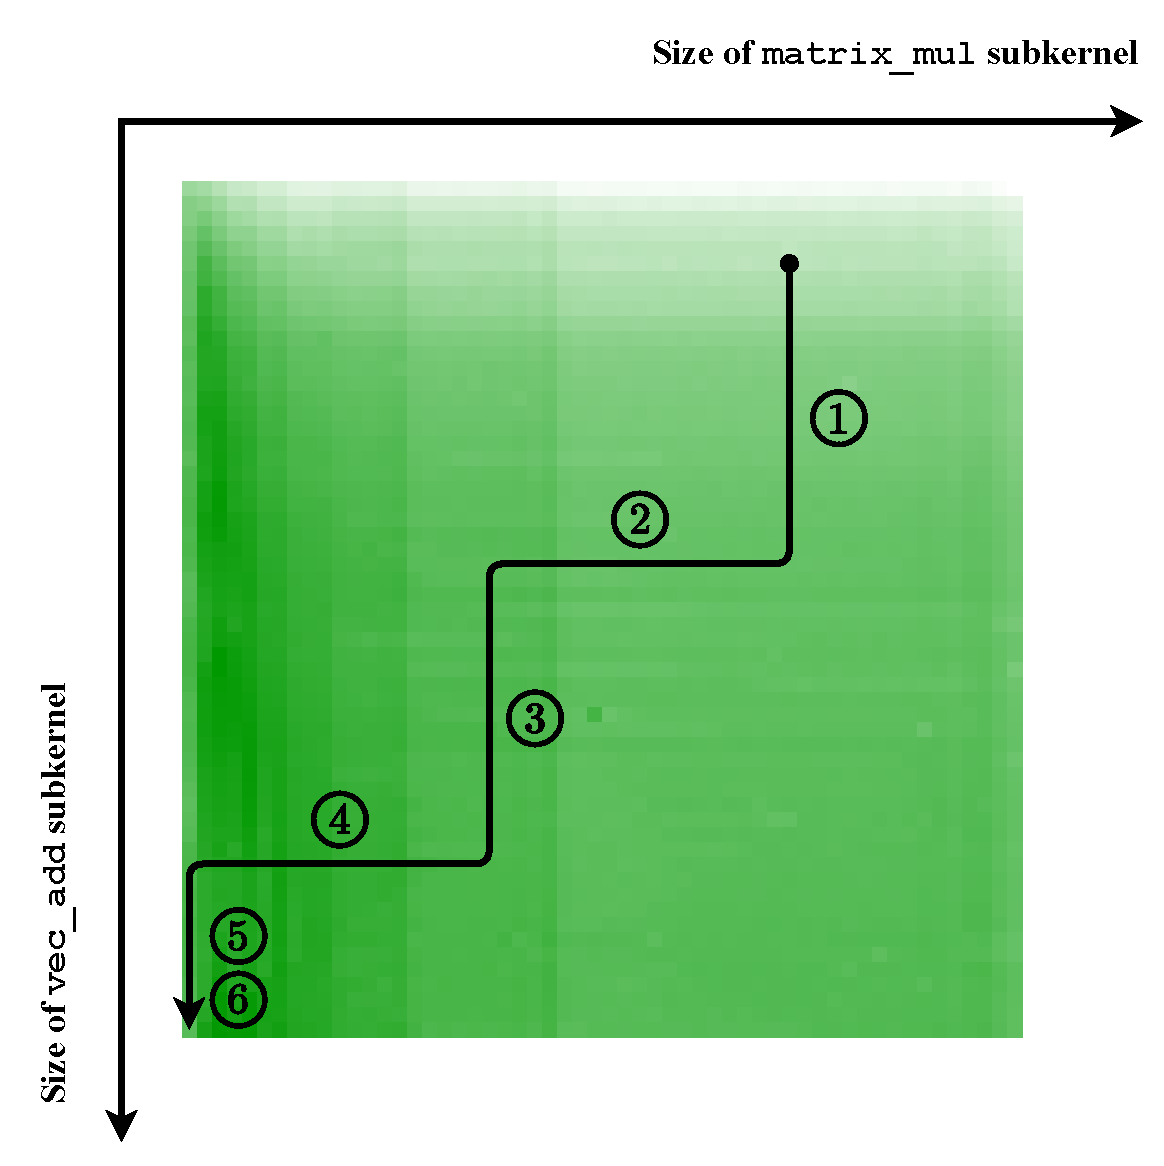
\includegraphics[width=0.8\linewidth]{searching_trace/searching_trace_va_mm.drawio.pdf}
    \caption{搜索步骤示意图。其中5、6两步方向相同,但步长不同。}
    \label{searching-trace}
\end{figure}

为解决以上问题,ko-Sched搜索时采用可变步长。在搜索初期,使用较大步长快速定位至性能高的参数区域,避免受困于初始位置周边的局部最优解;之后以小步长在此区域寻找精准优解。\autoref{searching-trace} 展示了\texttt{matrix\_mul}和\texttt{vec\_add}联合调度时算法给出的结果:1-4步使用较大步长减少迭代次数,5-6步(第5、6步方向相同)使用较小步长寻找区域内最优解。

此外,为减少迭代次数,ko-Sched不以单个block为subkernel调整的最小单位,而是限定了步长的最小值。对于具有$S$个SM,每个SM具有$P$个CUDA核心的GPU设备,对于每个block具有$"block\_size"$个线程的kernel,最小调整单位设置为
\begin{equation}
    S \times \max \left(\left\lceil \frac{P}{\text{block\_size}}\right\rceil  , 1\right) \text{blocks} \label{eq:searching:stepsize}
\end{equation}
此数值为满足以下条件的最小值:
\begin{enumerate*}[label=\roman*),itemjoin={\quad}]
    \item 每个SM均分配有至少1个block
    \item 每个SM的CUDA核心数目不少于此SM上分配有的线程数目。
\end{enumerate*}

最后,ko-Sched根据kernel的单一block任务量为kernel设置不同的步长。本文的实验中视各kernel具有相似的总任务量,故设定block数目较多的kernel的单一block任务量小,对其设置较长步长。我们将对此策略的改进留作后期工作。

\subsection{多个初始配置的搜索}

\begin{algorithm}[htbp]
    \SetAlgoLined
    \KwData{初始分割参数列表 init\_config\_list}
    \KwResult{搜索所得性能最佳分割参数}
    min\_exec\_time $\gets$ \textbf{inf}\; \label{algo:searching-mult-init:initmin}
    min\_exec\_config $\gets$ \textbf{null}\; \label{algo:searching-mult-init:initminconfig}
    \ForEach{init\_config $\in$ init\_config\_list}{
        exec\_time $\gets$ subkernel\_size\_search(init\_config)\; \label{algo:searching-mult-init:profiletime}
        \If{exec\_time $<$ min\_exec\_time}{
            min\_exec\_time $\gets$ exec\_time\; \label{algo:searching-mult-init:updatemin}
            min\_exec\_config $\gets$ config\; \label{algo:searching-mult-init:updateconfig}
        }
    }
    \Return{min\_exec\_config}\;
    \caption{Subkernel Size Searching with Multiple Initial Configurations}
    \label{algo:searching-mult-init}
\end{algorithm}

尽管可变步长降低了算法收敛于局部最优解的可能,在我们的实验中仍出现了所得结果显著劣于理论最优解的情况。因此,ko-Sched会选取多个初始配置依次进\autoref{algo:searching}中的搜索操作,并选择结果中最优者。如\autoref{algo:searching-mult-init}所示,算法对\texttt{init\_config\_list}中的初始配置依次调用\autoref{algo:searching}(\autoref{algo:searching-mult-init:profiletime},函数\texttt{subkernel\_size\_search}),并记录搜索结果中性能最好的配置(\autoref{algo:searching-mult-init:updateconfig})。

\section{分割配置的性能分析}\label{sec:profile}

\autoref{algo:searching}中另一常用操作是用于估算特定配置下的程序性能的\texttt{estimate\_exec\_time}函数,此函数的效率对整个搜索算法的执行时间有重要影响。Ko-Sched通过测量2个kernel的部分子内核并行执行时间估算整个程序的运行时长。具体而言,设在某分割参数下,内核1具有$N_1$数目的子内核,内核2具有$N_2$数目的子内核,则ko-Sched会分别启动$\left\lceil \frac{N_1}{C}\right\rceil $和$\left\lceil \frac{N_2}{C}\right\rceil $个内核1和内核2的子内核,并视其执行时间的$C$倍为估算得的全程执行时间。其中$C$为一个与内核1、内核2有关的常数,用于平衡测量开销和测量结果的准确性。\autoref{sampling}展示了$C=N_1$时估算kernel 1和kernel 2并行性能的情形。每一实线矩形代表一子内核($SubK_{i}$),其中彩色矩形指测量时执行的子内核,灰色矩形指不会执行的子内核。图中kernel 1启动了1个子内核,与kernel 2的5个子内核联合调度。经实验,ko-Sched将$C$的默认值设定为$2 \times \min \left(N_1, N_2\right)$。

\begin{figure}[htbp]
    \centering
    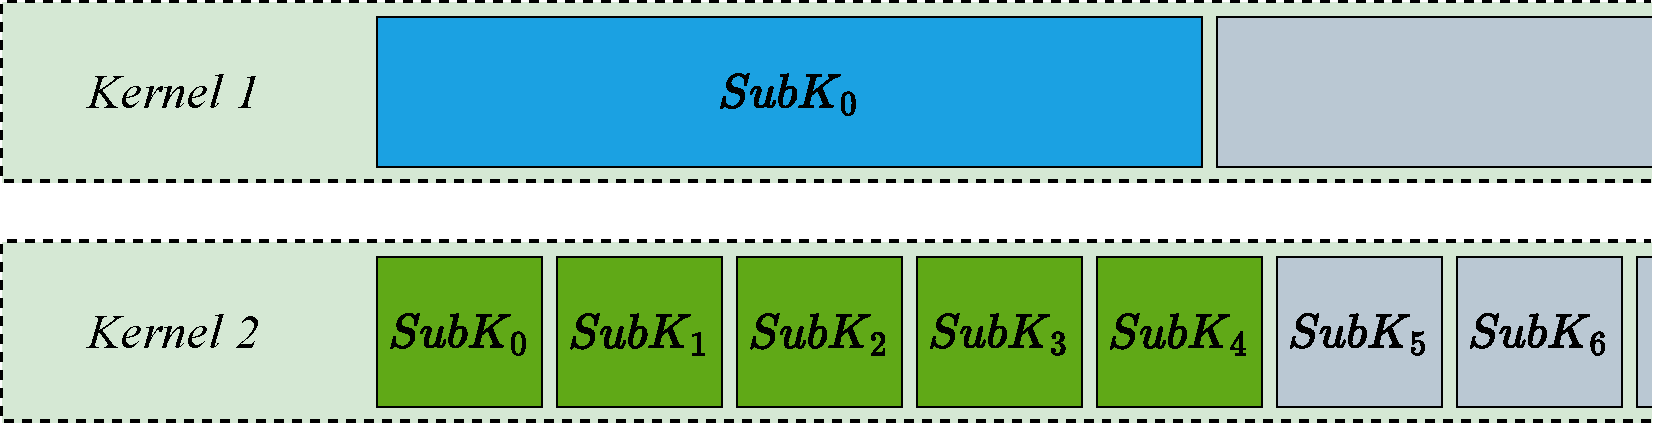
\includegraphics[width=0.8\linewidth]{sampling/sampling.drawio.pdf}
    \caption{测量子内核并行执行时间的示意图}
    \label{sampling}
\end{figure}

\autoref{evaluation}\autoref{exp-est}展示了$C=2 \times \min \left(N_1, N_2\right)$时性能估算的影响。尽管对性能的估算影响了搜索算法结果的准确性,但与通过准确计时获得的结果相差较小,且大大降低了搜索的执行时间。